\begin{enumerate}
 \item\begin{enumerate}
 \item Pour la symétrie par rapport à $(Ox)$, chacune des distances à $A$ et $B$ est conservée car $A$ et $B$ sont sur l'axe de symétrie. La courbe $(C)$ est donc conservée. Pour la symétrie par rapport à $(Oy)$, les points $A$ et $B$ sont échangés. Lorsque $M\in (C)$ les distances sont échangées et le produit est conservé. La courbe $(C)$ est donc conservée.
\item On écrit simplement les distances avec des coordonnées. Comme tout est positif, l'équation devient :
\begin{multline*}
 \left( (x-a)^2+y^2\right)\left( (x+a)^2+y^2\right)=k^4 \\ \Leftrightarrow
\left(x^2+y^2+a^2-2ax \right)\left(x^2+y^2+a^2+2ax \right)=k^4 \\ \Leftrightarrow
(x^2+y^2+a^2)^2 -4a^2x^2=k^4 
\end{multline*}
Il ne semble pas utile de développer.
\item Lorsqu'on passe en coordonnées polaires $x=\rho\cos \theta$, $y=\rho\sin \theta$ avec $\rho>0$, l'équation devient
\begin{displaymath}
 (\rho^2+a^2)^2-4a^2\rho^2 \cos^2\theta = k^4
\end{displaymath}
\end{enumerate}
 
\item \begin{enumerate}
 \item On peut former une équation du second degré en $R$ qui redonne $(E)$ lorsque l'on substitue $\rho^2$ à $R$.
\begin{displaymath}
  (R+a^2)^2-4a^2R\cos\theta = k^4 \Leftrightarrow
R^2 +2a^2(1-2\cos^2\theta)R+a^4-k^4=0
\end{displaymath}On met finalement le trinôme sous la forme
\begin{displaymath}
  (1) \hspace{0.5cm} R^2 -2a^2\cos 2\theta\, R +a^4-k^4=0 
\end{displaymath}

\item L'équation $(1)$ admet deux solutions strictement positives (éventuellement confondues) si et seulement si
\begin{itemize}
 \item le discriminant $\Delta$ est positif ou nul
 \item le produit $P$ des racines est strictement positif (elles sont de même signe)
 \item la somme $S$ des racines est strictement positive
\end{itemize}
Après calcul, on obtient donc un système de trois conditions.
\begin{displaymath}
 \left\lbrace 
\begin{aligned}
 \Delta = 4(k^4-a^4\sin^2 2\theta) &\geq 0 \\
 P = a^4-k^4 &>0\\
 S = 2a^2\cos2\theta &>0
\end{aligned}
\right. 
\end{displaymath}
Comme $a$ et $k$ sont strictement positifs, la condition sur le produit donne $k<a$. Avec l'hypothèse $\theta\in[0,\frac{\pi}{2}]$, la condition sur la somme devient $\theta\in[0,\frac{\pi}{4}]$. De plus $\sin 2\theta \geq 0$ et la condition sur le discriminant devient $\sin2\theta\leq \frac{k^2}{a^2}$. Finalement, les trois conditions se réduisent donc à deux :
\begin{displaymath}
 \left\lbrace 
\begin{aligned}
k &<a\\
\theta &\in \left[0,\dfrac{1}{2}\arcsin\dfrac{k^2}{a^2}\right]
\end{aligned}
\right. 
\end{displaymath}
\begin{figure}[ht]
 \centering
 \input{Clemn_1.pdf_t}
 \caption{Cas $a=1$, $k=0.9$. Courbes polaires $r_1$ et $r_2$.}
 \label{Clemn_1}
\end{figure}

\item Lorsque $k<a$, les $\theta$ pour lesquels le discriminant est positif sont entre $0$ et $\frac{1}{2}\arcsin\dfrac{k^2}{a^2}$. Dans ce cas, le trinôme en $R$ admet deux solutions positives
\begin{align*}
 a^2\cos^2\theta + \sqrt{k^4-a^4\sin^2 2\theta} & & a^2\cos^2\theta - \sqrt{k^4-a^4\sin^2 2\theta} 
\end{align*}
La courbe $(\tilde{C})$ est donc le support des deux courbes paramétrées (voir figure \ref{Clemn_1}):
\begin{displaymath}
 \theta \in \left[0,\dfrac{1}{2}\arcsin\dfrac{k^2}{a^2}\right]:\hspace{.3cm}
\left\lbrace
\begin{aligned}
 r_1(\theta) &= \sqrt{a^2\cos 2\theta + \sqrt{k^4-a^4\sin^2 2\theta}} \\
 r_2(\theta) &= \sqrt{a^2\cos 2\theta - \sqrt{k^4-a^4\sin^2 2\theta}}
\end{aligned}
 \right. 
\end{displaymath}

\item Dans le cas où $k>a$. Les droites de pente négatives ne coupent pas le quart de plan, elles ne peuvent donc pas couper la courbe. Pour les droites de pente positive on est ramené à l'éyude précédente.\\
Le produit des deux racines devient négatif, la somme reste positive et le discriminant est positif pour tous les $\theta$. Le trinôme admet toujours deux racines mais une seule est positive. Il existe donc un seul point d'intersection. La courbe complète prend une forme de cacahuète.
\end{enumerate}

\item \begin{enumerate}
 \item Si $k=a$, le terme constant dans l'équation cartésienne disparait, on peut simplifier par $r^2$ et il reste (comme $r>0$):
\begin{displaymath}
 r=a\sqrt{2\cos(2\theta)}
\end{displaymath}
Cette courbe est appelée \emph{lemniscate}.
\item Si $k=a=\frac{1}{\sqrt{2}}$, la courbe paramétrée s'écrit
\begin{displaymath}
 M(\theta) = O + \sqrt{\cos2\theta}\overrightarrow{e}_\theta
\end{displaymath}
La vitesse se factorise bien :
\begin{multline*}
 \overrightarrow{M'}(\theta)
=-\dfrac{\sin 2\theta}{\sqrt{\cos2\theta}}\overrightarrow{e}_\theta +\sqrt{\cos2\theta}\overrightarrow{e}_{\theta +\frac{\pi}{2}}\\
=\dfrac{1}{\sqrt{\cos2\theta}}\left( -\sin 2\theta \overrightarrow{e}_\theta + \cos 2\theta\overrightarrow{e}_{\theta +\frac{\pi}{2}}\right) \\
=\dfrac{1}{\sqrt{\cos2\theta}}\left(  \cos 2\theta\overrightarrow{e}_{\theta +\frac{\pi}{2}} +\sin 2\theta \overrightarrow{e}_{\theta+\frac{\pi}{2}+\frac{\pi}{2} }\right)
= \dfrac{1}{\sqrt{\cos2\theta}}\overrightarrow{e}_{3\theta +\frac{\pi}{2}}
\end{multline*}
Examinons les symétries: $M(-\theta)$ est le symétrique de $M(\theta)$ par rapport à l'axe $Ox$ et $M(\theta +\Pi)$ est le symétrique de $M(\theta)$ par rapport à $O$.\newline
On se limite donc au premier quart de plan. On doit alors avoir $\theta$ compris entre $0$ et $\frac{\pi}{4}$ pour assurer la positivité du $\cos2\theta$. La fonction $r$ décroît de $1$ à $0$. Les directions des tangentes se tracent facilement avec la formule du dessus. On remarque que la fonction n'est pas dérivable en $\frac{\pi}{2}$. La vitesse devient infinie mais le vecteur unitaire de sa direction tend vers $\overrightarrow{e}_{\frac{5\pi}{4}}$. Le tracé de ce quart de courbe est présenté en figure \ref{fig:Clemn_2}, il est à compléter par symétrie.
\end{enumerate}
\begin{figure}
 \centering
 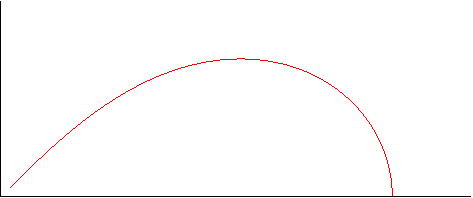
\includegraphics{Clemn_2.pdf}
 % Clemn_2.pdf: 275x115 pixel, 72dpi, 9.70x4.06 cm, bb=0 0 275 115
 \caption{Tracé d'un quart de lemniscate}
 \label{fig:Clemn_2}
\end{figure}

\end{enumerate}
